\documentclass[10pt,a4paper]{article}
\usepackage[utf8]{inputenc}
\usepackage[frenchb]{babel}
\usepackage[T1]{fontenc}
\usepackage{amsmath}
\usepackage{amsfonts}
\usepackage{amssymb}
\usepackage{lmodern}
\usepackage{graphicx}

\begin{document}

\subsection*{Question 7 (Ivan)}

\paragraph*{Pouvez-vous déterminer précisément de quelle variante de table de hachage la classe Java.util.Hashtable s'agit?}
\\
La classe java.util.Hashtable est une AbstractHashMap. 

\paragraph{Java fournit-il d'autres implémentations de l'interface Map? Faites un diagramme qui représente les interfaces et les classes qui se rapportent à map et précisez ce qui les caractérise.}

-Interface Map\\
-Classe AbstractMap : l'AbstractMap est un type abstrait de données qui représente une collection de paires clef-valeur et qui implémente l'interface Map.\\
-Classe UnsortedTableMap : La classe UnsortedTableMap étend la classe AbstractMap et correspond à une table dont les éléments de la collection ne sont pas ordonnés, ce qui implique un manque d'efficacité dû au fait que chaque méthode a une complexité linéaire au maximum au lieu d'être constante car il faut scanner tous les éléments pour trouver une entrée. \\
-Classe AbstractHashMap : La classe AbstractHashMap étend la classe AbstractMap. La principale différence est que les tables de hachages peuvent avoir des clés qui ne sont pas des entiers mais qui peuvent être des symboles.  \\ 
-Classe ChainHashMap : Cette classe étend la classe AbstractHashmap et utilise le chainage de sorte que toutes les valeurs ayant la même clef soient regroupés dans une structure chainée. Cela permet d'éviter les collisions.\\
-Classe ProbeHashMap : Cette classe étend la classe AbstractHashMap et utilise aussi un système permettant d'éviter les collisions. Le système est tel que si l'on veut insérer un élément dans la table mais qu'une clef possède déjà une valeur, on essaye d'insérer la valeur à la clef suivante, et ainsi de suite jusqu'à trouver une clef non-occupée. \\ 
\\
-Interface SortedMap : L'interface SortedMap étend l'interface Map. La particularité de SortedMap est que les valeurs sont mappés de sorte qu'ils soient ordonnés.\\
-Classe AbstractSortedMap : Il s'agit d'un type abstrait de données qui représente une collection ordonnée de paires clef-valeur. Cette classe implémente l'interface SortedMap.\\
-Classe SortedTableMap : Cette classe étend la classe AbstractSortedMap et correspond à une table dynamique dans laquelle sont stockées les entrées dans un ordre croissant selon la valeur des clefs. Grâce à cette structure la recherche binaire est possible.  \\
-Classe TreeMap : Cette classe permet de représenter les valeurs sous forme hiérarchique. \\ 

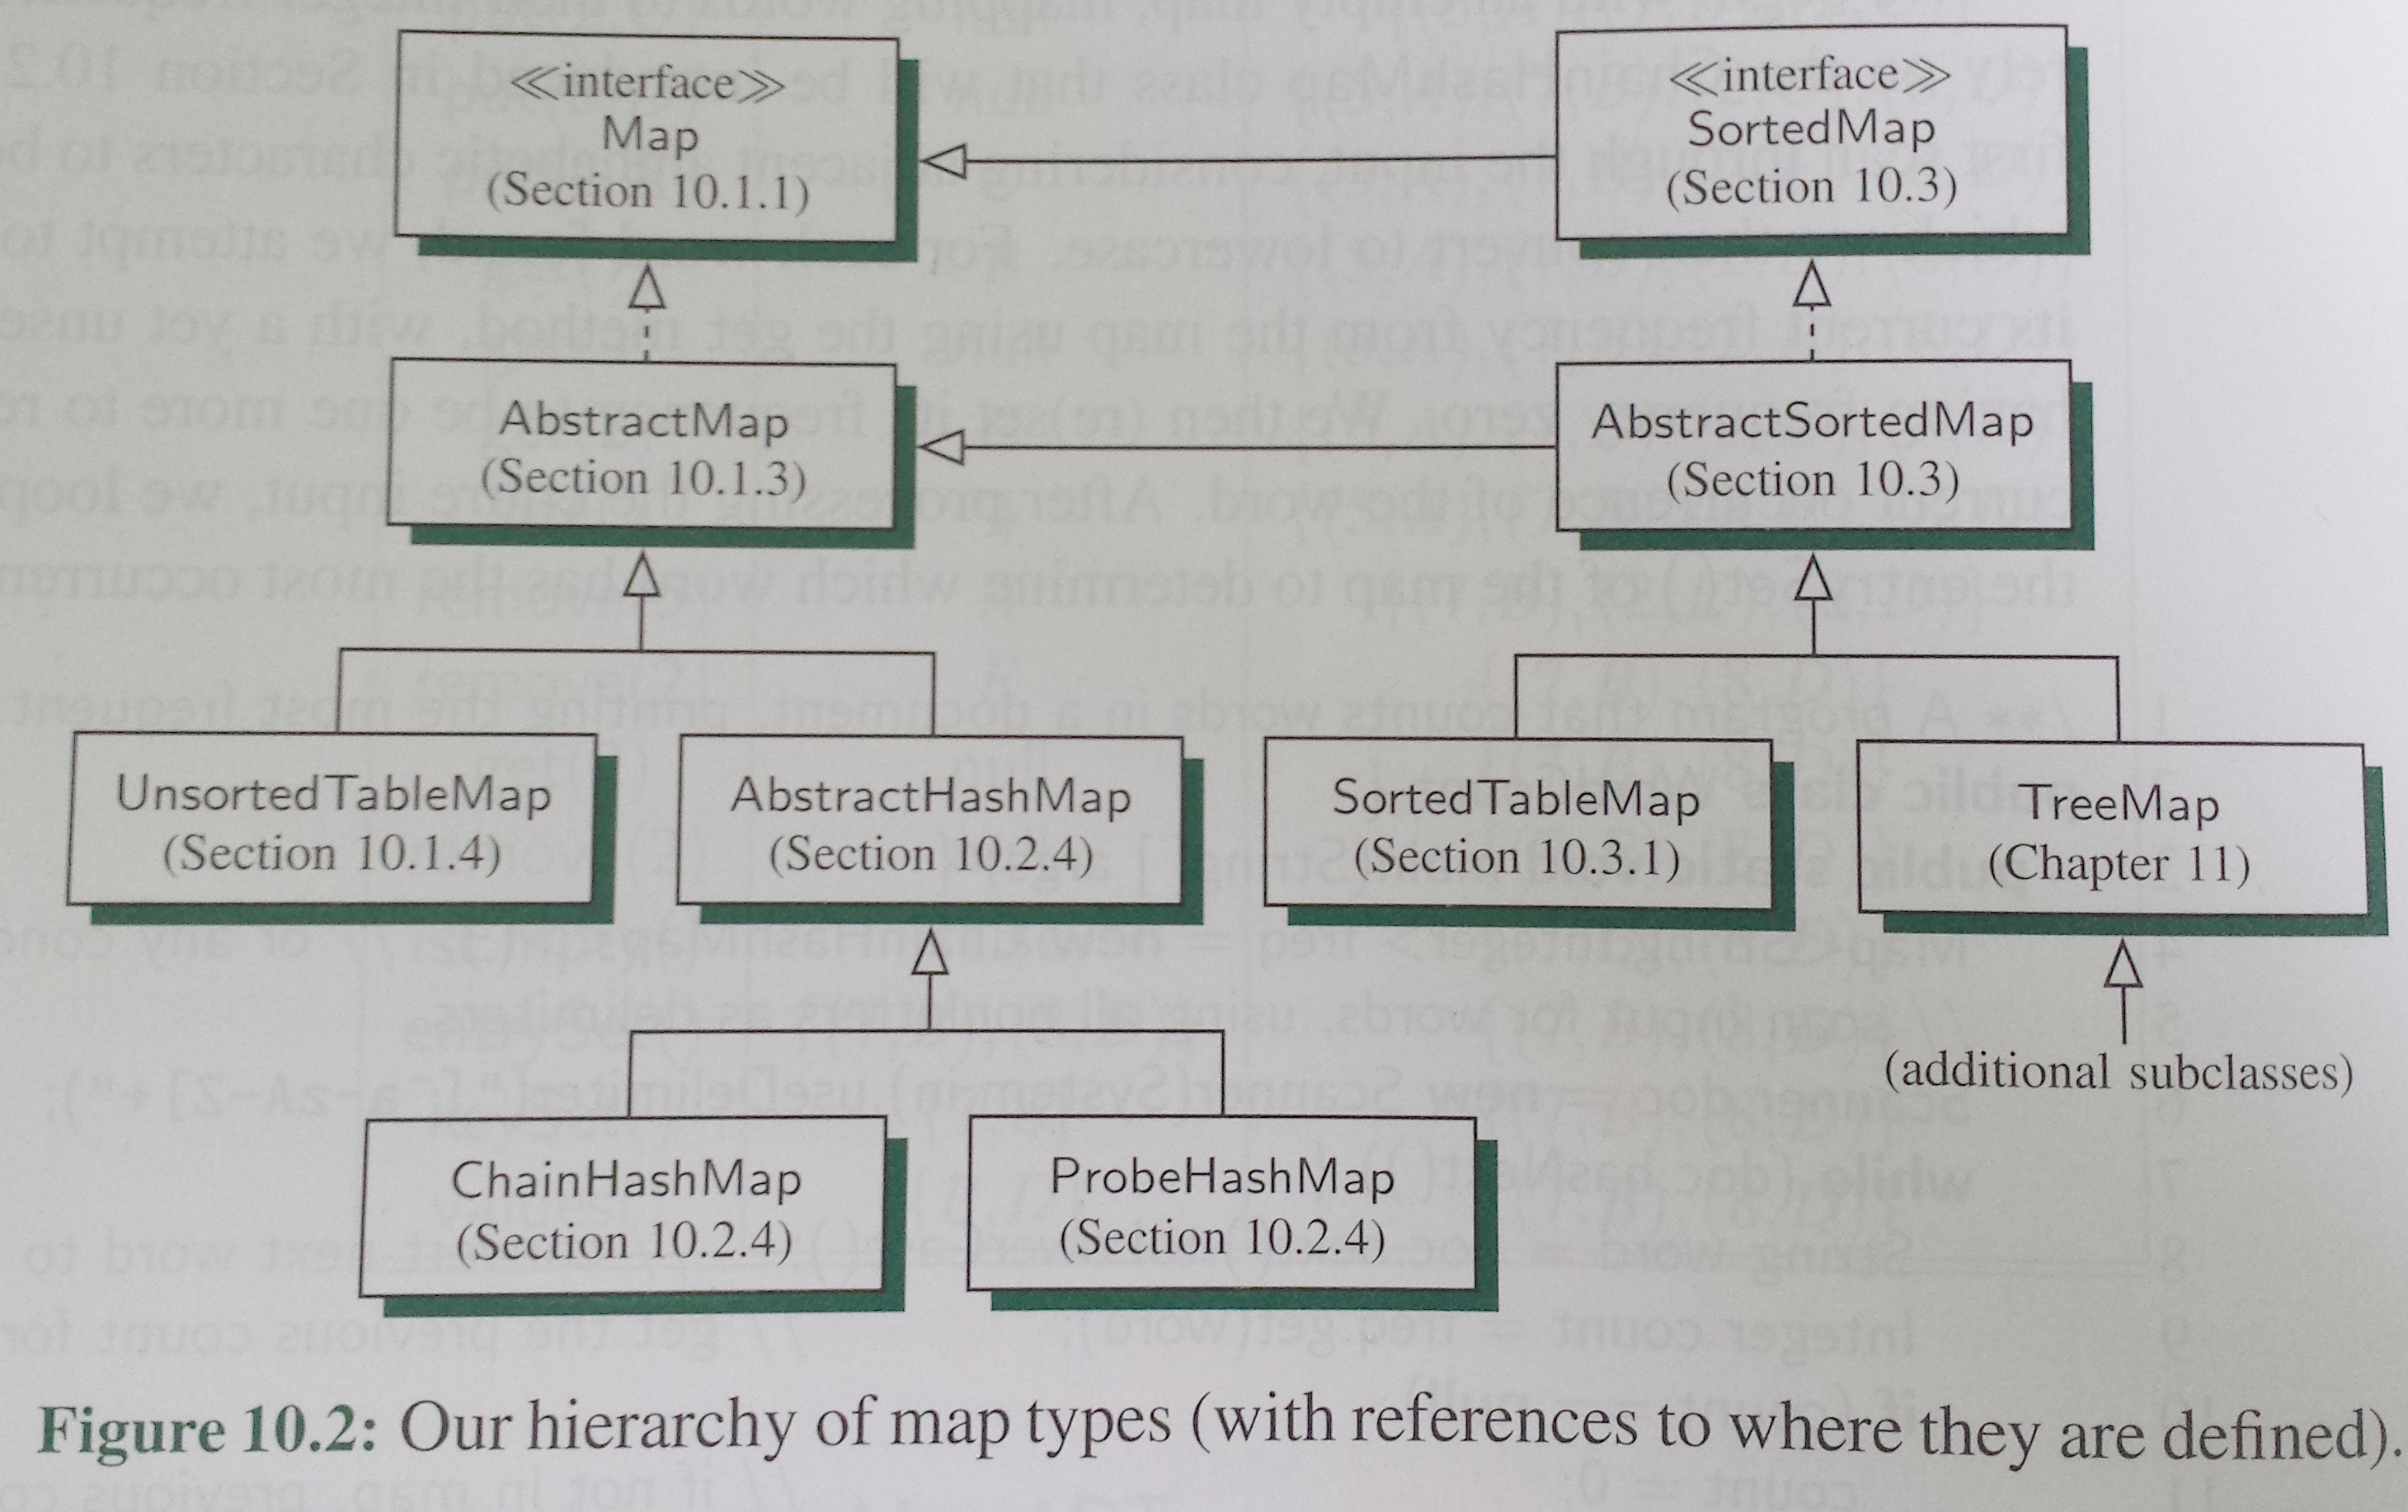
\includegraphics[scale=0.3]{diagramme.png}
\\
==> Diagramme représentant les classes et interfaces se rapportant à Map. \\
(Source : DSAJ6, page 374)\\

\paragraph{Qu'est-ce qui peut servir de clef pour une hashtable en Java?}
\\
Les chaines de caractères peuvent servir de clef en Java car il s'agit d'un type plus général que les caractères ou les entiers. Ainsi on peut utiliser plus de symboles pour définir les clefs. 

\end{document}